%!TEX encoding = UTF8
%!TEX root =notes.tex

\section{Géométrie plane}\label{sec:geom-plane}

Sur la droite réelle, on associe chaque point avec un nombre, appelé nombre réel : chaque point correspond à un nombre, et chaque nombre correspond à un point.

Dans cette section, on augmente la notion de droite réelle en ajoutant une dimension ; la droite devient le plan.
On associera alors à chaque point du plan \emph{deux}\footnote{Il s'avère qu'il est possible en théorie d'associer chaque point du plan à un unique nombre, mais la construction dépasse le champ d'application de ce cours.} nombres réel : le premier représentant sa position \og gauche/droite \fg et le deuxième sa position \og haut/bas \fg.

Un point sera alors un couple $(x,y)$ où $x,y \in \R$ sont deux nombres réels appelés respectivement l'abscisse et l'ordonnée du point.

\subsection{Repère orthonormé}

\dfn{Repère}{
	
	\begin{multicols}{2}

	Un repère est determiné par trois points $(O; I,J)$ comme ci-contre.
	\begin{itemize}
		\item Le point $O$ est appelé l'\textbf{origine}.
		\item La droite $(OI)$ est appelée l'axe des \textbf{abscisses}.
		\item La droite $(OJ)$ est appelée l'axe des \textbf{ordonées}.
		\item[]
		\item[]
	\end{itemize}
	
	
	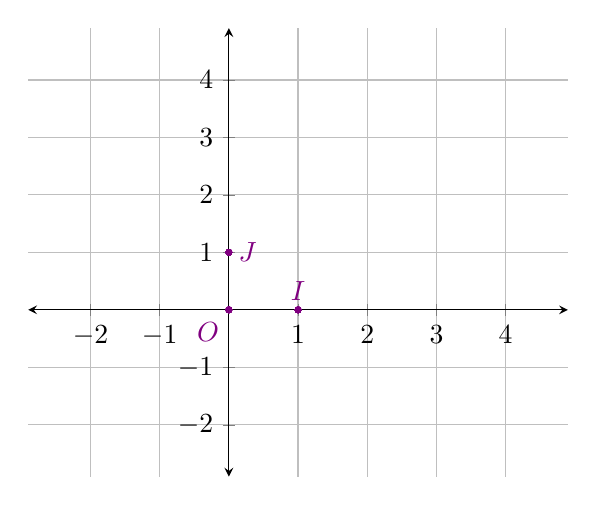
\begin{tikzpicture}[>=stealth, scale=1]
		\begin{axis}[xmin = -2.9, xmax=4.9, xtick={ -3, ..., 5}, ymin=-2.9, ymax=4.9, ytick={-3, ..., 5}, axis x line=middle, axis y line=middle, axis line style=<->, xlabel={}, ylabel={}, grid=both]
		
			\addplot[violet, mark=*, mark size = 1] (0,0) node[below=8pt, left] {$O$};
			\addplot[violet, mark=*, mark size = 1] (1,0) node[above] {$I$};
			\addplot[violet, mark=*, mark size = 1] (0,1) node[right] {$J$};
		\end{axis}
	\end{tikzpicture}
	\end{multicols}

}{}

\dfn{Repère orthonormé}{
	Un repère $(O; I, J)$ est
	\begin{enumerate}
		\item \textbf{orthogonal} si ses axes $(OI)$ et $(OJ)$ sont perpendiculaires ;
		\item \textbf{normé} si les segments $[OI]$ et $[OJ]$ sont de même longueur (fixée à $1$) ;
		\item \textbf{orthonormé} s'il est orthogonal et normé.
	\end{enumerate}´
}{def:repere-orthonorme}

\nt{
	L'ordre des points $I$ et $J$ est important car il donne l'ordre de lecture des coordonnées.
	Traditionnellement, l'axe des abscisse est horizontale, et celle des ordonnée verticale.
	
	Ainsi, le point $I$ admet pour coordonnée $(1;0)$, et le point $J$ $(0;1)$.
	On notera alors :
		\begin{align*}
			I(1;0), && \text{ et } && J(0;1).
		\end{align*}
}

\ex{}{
	\begin{multicols}{2}
		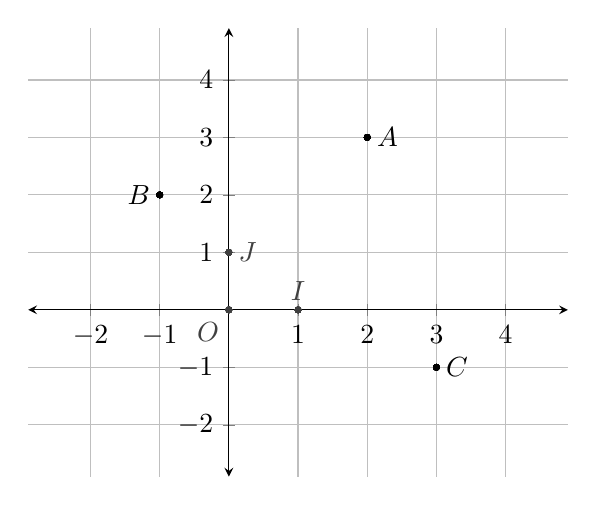
\begin{tikzpicture}[>=stealth, scale=1]
		\begin{axis}[xmin = -2.9, xmax=4.9, xtick={ -3, ..., 5}, ymin=-2.9, ymax=4.9, ytick={-3, ..., 5}, axis x line=middle, axis y line=middle, axis line style=<->, xlabel={}, ylabel={}, grid=both]
		
			\addplot[darkgray, mark=*, mark size = 1] (0,0) node[below=8pt, left] {$O$};
			\addplot[darkgray, mark=*, mark size = 1] (1,0) node[above] {$I$};
			\addplot[darkgray, mark=*, mark size = 1] (0,1) node[right] {$J$};
			
			\addplot[black, mark=*, mark size = 1] (2,3) node[above, right] {$A$};
			\addplot[black, mark=*, mark size = 1] (-1,2) node[above, left] {$B$};
			\addplot[black, mark=*, mark size = 1] (3,-1) node[below, right] {$C$};
		\end{axis}
	\end{tikzpicture}
	
	Les points $A$, $B$, et $C$ admettent pour coordonnées, dans le repère $(O; I, J)$,
		\begin{align*}
			A(2;3), && B(-1;2), && C(3;-1).
		\end{align*} 
	\end{multicols}
}{}

\nt{
	On omettera parfois de préciser que le repère est orthonormé.
	
	On voit donc le plan comme l'ensemble des couples de réels :
		\[ \{ (x, y) \text{ tq. } x \in \R, \text{ et } y\in\R \}. \]
}


\subsection{Segments du plan : longueur et milieu}\label{sec:longueur-milieu}

\dfn{Segment}{
	Soient $E, F$ deux points du plan. Le segment $[EF]$ est l'ensemble des points de la droite $(AB)$ situés entre $A$ et $B$ (tous les deux inclus).
}{deg:segment}

\nt{
	Un segment du plan est une généralisation d'un intervalle sur la droite.
	Tous les segments du plans qui seront considérés contiennent leur bornes (contrairement aux intervalles !).
}

\mprop{}{
	Soient $a,b \in \R$ deux nombres réels tels que $a < b$.
	
	Alors le milieu de l'intervalle $[a,b]$ est égal à $\dfrac{a+b}2$.
}{prop:milieu-inter}

\pf{Démonstration de la proposition \ref{prop:milieu-inter}}{
	Notons $x\in\R$ le milieu de l'intervalle.
	Celui-ci est à équidistance de $a$ et de $b$ et vérifie donc
		\[ |x-a| = |x-b|. \]
	Comme $x$ vérifie $a \leq x \leq b$, et par définition de la valeur absolue, on a
		\begin{align*}
			|x-a| &= x-a, \text{ et} \\
			|x-b| &= -(x-b) = b-x.
		\end{align*}
	On peut alors résoudre pour $x\in\R$ :
		\begin{align*}
			x-a = b-x && \iff && 2x = a+b && \iff && x = \dfrac{a+b}2
		\end{align*}
}

\nt{
	En voyant $\dfrac{a+b}2$ comme $\dfrac12 a + \dfrac12 b$, on peut comprendre le milieu comme une moyenne de deux valeurs ($a$ et $b$).
	C'est d'ailleurs comme ça qu'on calcule une moyenne de notes ayant le même coefficient -- leur poids est alors $\dfrac12$.
	Remarquons que la somme des poids vaut toujours $1$ : ils correspondent aux coefficients divisés par la somme de tous les coefficients.
	
	En changeant les poids, on peut créer d'autres points de l'intervalle. 
	Par exemple, si $a$ compte deux fois plus que $b$, les coefficients seront (par exemple) $2$ et $1$, et les poids $\dfrac23$ et $\dfrac13$.
	 La formule de la moyenne pondérée sera alors
		\[ \dfrac23a + \dfrac13b, \]
	qui est plus proche de $a$ que de $b$.
}

\exe{}{
	Considérons l'intervalle $[15;20]$ qui correspond à deux notes : $15$ et $20$.
	\begin{enumerate}
		\item Si les deux notes ont le même coefficient fixé à $1$, quel est le poids de chaque note et quelle est la moyenne pondérée ? Comparer avec le milieu de l'intervalle.
		\item Posons $\lambda \in [0;1]$ le poids de la première note, et $1-\lambda$ celui de la deuxième.
			Calculer la moyenne pondérée $15\lambda + 20(1-\lambda)$ pour certaines valeurs de $\lambda$ dans son intervalle $[0;1]$. 
			Vérifier que toutes les valeurs obtenues appartiennent bien à l'intervalle $[15;20]$.
		\item Quel $\lambda \in [0;1]$ choisir pour avoir une moyenne de $18{,}5$ ?
	\end{enumerate}
}{exe:milieu-inter}

\mprop{}{
	Soient $A(x_A, y_B)$ et $B(x_A,y_B)$ deux points du plan.
	
	Alors le milieu du segment $[AB]$ est le point $M$ de coordonnées
		\begin{align}\label{expr:milieu}
			M\left(\dfrac{x_A+x_B}2, \dfrac{y_A + y_B}2\right).
		\end{align}
}{prop:milieu-segment}

\pf{Démonstration de la proposition \ref{prop:milieu-segment}}{

	Le point $M$ est au centre du rectangle dont les coins sont $A$ et $B$.
	Ainsi ses coordonnées sont les moyennes des coordonnées et $A$ et de $B$.
	
	\centering
	\resizebox{8cm}{!}{
	\begin{tikzpicture}[>=stealth, scale=1.2]
		\begin{axis}[xmin = -6.9, xmax=22.9, xticklabel=\empty, ymin=-2.9, ymax=4.9, yticklabel=\empty, axis x line=middle, axis y line=middle, axis line style=<->, xlabel={}, ylabel={}]
		
			% A and B
			\addplot[black, mark=*, mark size = 1] (1,3) node[above, right] {$A$};
			\addplot[black, mark=*, mark size = 1] (20,-2) node[below, right] {$B$};
			
			
			\addplot[black, thick, mark=|, mark size = 4] (1,0) node[below] {$x_A$};
			\addplot[black, thick, mark=|, mark size = 4] (20,0) node[above] {$x_B$};
			\addplot[black, thick, mark=-, mark size = 4] (0,3) node[left] {$y_A$};
			\addplot[black, thick, mark=-, mark size = 4] (0,-2) node[left] {$y_B$};
			
			% midpoint
			\addplot[red, mark=*, mark size = 1] (10.5,.5) node[above=10pt, right] {$M$};	
			\addplot[red, thick, mark=|, mark size = 4] (10.5,0) node[below=3pt] {$\dfrac{x_A+x_B}2$};
			\addplot[red, thick, mark=-, mark size = 4] (0,.5) node[above=3pt, left] {$\dfrac{y_A+y_B}2$};
			
			
			\draw[red, dotted, thick] (axis cs:10.5, 0) -- (axis cs:10.5,.5);
			\addplot[red, dotted, thick, domain = 0:10.5, samples=2] {.5};
			
			% dotted rectangle
			\draw[black, dotted, thick] (axis cs:1, 0) -- (axis cs:1,3);
			\draw[black, dotted, thick] (axis cs:20, 0) -- (axis cs:20,-2);
			\addplot[black, dotted, thick, domain = 0:1, samples=2] {3};
			\addplot[black, dotted, thick, domain = 0:20, samples=2] {-2};
		
			
		\end{axis}
	\end{tikzpicture}
	}
	
}

\nt{
	La formule \eqref{expr:milieu} du milieu du segment $[AB]$ ressemble de près à celle du milieu d'un intervalle.
	Pour simplifier les expressions, il sera alors pratique d'écrire
		\[ M = \dfrac{A+B}2 = \dfrac12 A + \dfrac12 B.\]
	Pour cela, il faut pouvoir additionner les points du plans, et les multiplier par des nombres réels.
}

\dfn{Manipulations des points}{
	Soient $A(x_A, y_A)$, $B(x_B, y_B)$ deux points du plan et $\kappa \in \R$ un nombre réel quelconque.
	
	Les opérations suivantes sont légales.
		\begin{enumerate}
			\item L'addition de deux points : $A+B$, de coordonées $(x_A+x_B, y_A+y_B)$.
			\item La multiplication d'un point par un réel : $\kappa A$, de coordonnées $(\kappa x_A; \kappa y_A)$.
		\end{enumerate}
	\textbf{Attention} : on ne multiplie jamais les points ensemble ! Le produit $A$ par $B$ n'a pas de sens.
}{def:manip-points}


\ex{}{
	Considérons $A(1;3)$ et $B(-3;2)$ deux points du plan.
	Alors 
		\begin{multicols}{3}
		\begin{enumerate}
			\item $A+B = (-2 ; 5)$
			\item $·2B = (-6 ; 4)$
			\item $-A = (-1 ; -3)$
			\item $B - A = (-4 ; -1)$
			\item $-2A - B = (1 ; -8)$
			\item $\dfrac{A-2B}{2} = \left(\dfrac72 ; \dfrac{-1}2\right)$
		\end{enumerate}
		\end{multicols}
}{}

\mprop{Reformulation de la proposition \ref{prop:milieu-segment}}{
	Le milieu $M$ du segment $[AB]$ est égal à
		\[ M = \dfrac{A+B}{2}. \]
}{}

\nt{
	On peut retrouver la formule du milieu d'un intervalle en plongeant celui-ci dans le plan.
	Par exemple, l'intervalle $[-3;1]$ correspond au segment $[AB]$, où $A(-3;0)$ et $B(1;0)$.
	
	Le milieu $M$ du segment est alors $\dfrac{A+B}2 = (-1;0)$, qui correspond bien au milieu $\dfrac{-3+1}2 = -1$ de l'intervalle.
}

\exe{}{
	Représenter les points $A(1;1)$ et $B(3;-1)$ dans un repère orthonormé.
	Par analogie à avec l'exercice \ref{exe:milieu-inter}, représenter le point
		\[ \lambda A + (1-\lambda)B, \]
	pour certaines valeurs de $\lambda \in [0;1]$.
	
	Quel $\lambda$ choisir pour obtenir le point $C\left(\dfrac32; \dfrac12\right)$ ?
}{exe:milieu-segment}

\thm{Longueur d'un segment}{
	Soient $A(x_A, y_A)$, $B(x_B, y_B)$ deux points du plan dans un repère orthonormé.
	La longueur $\ell$ du segment $[AB]$ est donnée par
		\[ \ell = \sqrt{|x_A - x_B|^2 + |y_A - y_B|^2}. \]
}{thm:long-segment}

\pf{Démonstration du théorème \ref{thm:long-segment}}{
	Comme le repère est normé, on peut lire les distances sur les coordonnées.
	En particulier, la distance en la première coordonnée entre $A$ et $B$ est $|x_A - x_B|$.
	La distance en la deuxième coordonnée est $|y_A - y_B|$.
	On a donc le dessin suivant.
	
	\begin{center}
	\begin{tikzpicture}[>=stealth, scale=1.2]
		\begin{axis}[xmin = -1.9, xmax=15.9, xticklabel=\empty, ymin=-1.9, ymax=10.9, yticklabel=\empty, axis x line=middle, axis y line=middle, axis line style=<->, xlabel={}, ylabel={}]
		
			% A and B
			\addplot[black, mark=*, mark size = 1] (1,3) node[below] {$A$};
			\addplot[black, mark=*, mark size = 1] (10,8) node[below, right] {$B$};
			
			
			\addplot[black, mark=+, mark size = 1] (1,0) node[below] {$x_A$};
			\addplot[black, mark=+, mark size = 1] (10,0) node[below] {$x_B$};
			\addplot[black, mark=+, mark size = 1] (0,3) node[left] {$y_A$};
			\addplot[black, mark=+, mark size = 1] (0,8) node[left] {$y_B$};
			
			% triangle
			\draw[black, thick, decorate, decoration = {brace, mirror}] (axis cs:10,3) -- (axis cs:10,8) node [midway, right]{$|y_A-y_B|$};
			\draw[black, thick, decorate, decoration = {brace}] (axis cs:1, 3) -- (axis cs:10,8) node [midway, above=10pt, left]{$\ell$};
			\draw[black, thick, decorate, decoration = {brace, mirror}] (axis cs:1, 3) -- (axis cs:10,3) node [midway, below]{$|x_A-x_B|$};
			
		\end{axis}
	\end{tikzpicture}
	\end{center}
	
	Comme le repère est orthogonal, les axes sont perpendiculaires et le triangle est donc rectangle.
	Le théorème de Pythagore s'applique donc, et implique que
		\[ \ell^2 = |x_A-x_B|^2 + |y_A-y_B|^2, \]
	ce qui conclut.

}